\documentclass{article}
\usepackage[utf8]{inputenc}
\usepackage{multicol}
\usepackage{listings}
\usepackage{verbatim}
\usepackage{color}
\usepackage{geometry}
\usepackage{float}
\usepackage{amsmath}
\usepackage{caption}
\usepackage{pdflscape}
\usepackage{hyperref}
\setlength{\belowcaptionskip}{-10pt}
\setlength{\abovecaptionskip}{-30pt}
\floatstyle{boxed} 
\restylefloat{figure}
\usepackage{graphicx}
\definecolor{codegreen}{rgb}{0,0.6,0}
\definecolor{codegray}{rgb}{0.5,0.5,0.5}
\definecolor{codepurple}{rgb}{0.58,0,0.82}
\definecolor{backcolour}{rgb}{0.95,0.95,0.92}
\lstdefinestyle{mystyle}{
	backgroundcolor=\color{backcolour},   
	commentstyle=\color{codegreen},
	keywordstyle=\color{blue},
	numberstyle=\tiny\color{codegray},
	stringstyle=\color{codepurple},
	basicstyle=\footnotesize,
	breakatwhitespace=false,         
	breaklines=true,                 
	captionpos=b,                    
	keepspaces=true,                 
	numbers=left,                    
	numbersep=5pt,                  
	showspaces=false,                
	showstringspaces=false,
	showtabs=false,                  
	tabsize=2
}
\lstset{style=mystyle}
\title{Data Mining\\
		Home work 09\\Machine Learning Part:2 }
\author{Aqeel Labash\\ \textbf{Lecturer:} Jaak Vilo}
\date{06 April 2016}
\geometry{
	a4paper,
	total={170mm,257mm},	
	left=10mm,
	top=5mm,
}
\begin{document}
	\maketitle
\section*{First Question}
The article focus on classification. And here is the list 
\begin{itemize}
	\item No matter what algorithm you pick it's consist from three parts : Representation, Evaluation, Optimization.
	\item \textbf{Representation:} The feature we want to use in away computer can handle.
	\item \textbf{Evaluation or objective or scoring function:} used to distinguish between good and bad classifiers.
	\item \textbf{Optimization :} a method that search for best scoring classifiers.
	\item Generalization is what we want. "if there are 100,000 words in the dictionary, the spam filter described above has 2100,000 possible different inputs."
	\item Always test your module on data different than the train data.
	\item data by itself is not enough for generalization knowledge is also required to know which module to apply."A corollary of this is that one of the key criteria for choosing a representation is which kinds of knowledge are easily expressed in it. For example, if we have a lot of knowledge about what makes examples similar in our domain, instance-based methods may be a good choice. If we have knowledge about probabilistic dependencies, graphical models are a good fit.And if we have knowledge about what kinds of preconditions are required by each class, “IF . . . THEN . . .” rules may be the best option."
	\item \textbf{Over fitting} could be decomposed to Bias and Variance."Bias is a learner’s tendency to consistently learn the same wrong thing.Variance is the tendency to learn random things irrespective of the real signal." 
	\item Some ways to fight over fitting is: regularization term, cross validation, statistical significance.
	\item In most cases over fitting doesn't happen because of noise.
	\item intuitions used for low dimension usually don't  work with high dimension problems."our intuitions, which come from a three-dimensional world, often do not apply in high-dimensional ones."
	\item Numbers in theory might not be applicable and not always correct."consider the space of Boolean functions of d Boolean variables. If there are e possible different examples, there are \(2^e\) possible different functions, so since there are \(2^d\) possible examples,the total number of functions is \(2^{2^d}\).And even for hypothesis spaces that are “merely” exponential, the bound is still very loose, because the union bound is very pessimistic. For example, if there are 100 Boolean features and the hypothesis space is decision trees with up to 10 levels, to guarantee \(\delta = \epsilon = 1\%\) in the bound above we need half a million examples. But in practice a small fraction of this suffices for accurate learning."
	\item \textbf{Good Features:}are those which independent from each other and highly correlated with the class.
	\item Awesome feature is not necessarily provided by the data we might have to build it."Often, the raw data is not in a form that is amenable to learning, but you can construct features from it that are."
	\item The algorithm with more data wins."As a rule of thumb, a dumb algorithm with lots and lots of data beats a clever one with modest amounts of it. (After all, machine learning is all about letting data do the heavy lifting.)"
	\item The more data we have, the more complex the classifier.
	\item "Variable size learners can in principle learn any function given sufficient data, but in	practice they may not, because of limitations of the algorithm (for example,greedy search falls into local optima) or computational cost."
	\item Ensemble learning give better results usually.
	\item if the classifier is simpler doesn't mean it's more accurate.
	\item being able to represent the data doesn't mean that module can learn it."For example, standard decision tree learners cannot learn trees with more leaves than there are training examples."
	\item correlation doesn't mean one cause another.it's just an observation on the data that might have cause relation.
\end{itemize}
\section*{Second Question}
For this task I used the following Code : 
\begin{lstlisting}[language=Python]

# coding: utf-8

# In[72]:

get_ipython().magic(u'matplotlib inline')
import matplotlib.pyplot as plt


# In[4]:

original = {}
TotalPositive = 0
TotalNegative = 0
with open('data.class','r') as f:
f = f.readlines()
for line in f:
line = line.split()
if line[1]=='T':
original[line[0]]=True 
TotalPositive+=1
else:
original[line[0]]=False 
TotalNegative+=1
roc1=[]
with open('roc1.txt','r') as f:
f = f.readlines()
for line in f:
roc1.append(line.strip())
roc2=[]
with open('roc2.txt','r') as f:
f = f.readlines()
for line in f:
roc2.append(line.strip())
roc3=[]
with open('roc3.txt','r') as f:
f = f.readlines()
for line in f:
roc3.append(line.strip())
roc4=[]
with open('roc4.txt','r') as f:
f = f.readlines()
for line in f:
roc4.append(line.strip())


# In[41]:




# In[57]:

def GetTPFP(k,dataset):
TP=0
FP=0
TN=0
FN=0
for i in range (3000):
#Identified True
if i<k:
TP+=original[dataset[i]]
else:
TN+=original[dataset[i]]
#(TP,FP,TN,FN)
#(F11,F01,F10,F00)
#return (TP,TotalPositive-TP,TN,TotalNegative-TN)
return (float (TP)/float(TotalPositive),float(k-TP)/float(TotalNegative))



# In[58]:

roc1cm=[]
roc2cm=[]
roc3cm=[]
roc4cm=[]
print 'processing roc1'
for i in range (3000):
roc1cm.append(GetTPFP(i,roc1))
print 'processing roc2'
for i in range (3000):
roc2cm.append(GetTPFP(i,roc2))
print 'processing roc3'
for i in range (3000):
roc3cm.append(GetTPFP(i,roc3))
print 'processing roc4'
for i in range (3000):
roc4cm.append(GetTPFP(i,roc4))
print 'Finished'


# In[87]:

plt.figure('roc1.jpg')
plt.plot([x[1] for x in roc1cm],[x[0] for x in roc1cm], 'ro')
plt.ylabel('TPR')
plt.xlabel('FPR')
plt.title('Roc1')
#plt.show()
plt.savefig('roc1.jpg')


# In[86]:

plt.figure('roc2.jpg')
plt.plot([x[1] for x in roc2cm],[x[0] for x in roc2cm], 'ro')
plt.ylabel('TPR')
plt.xlabel('FPR')
plt.title('Roc2')
#plt.show()
plt.savefig('roc2.jpg')


# In[85]:

plt.figure('roc3.jpg')
plt.plot([x[1] for x in roc3cm],[x[0] for x in roc3cm], 'ro')
plt.ylabel('TPR')
plt.xlabel('FPR')
plt.title('Roc3')
#plt.show()
plt.savefig('roc3.jpg')


# In[82]:

plt.figure('roc4.jpg')
plt.plot([x[1] for x in roc4cm],[x[0] for x in roc4cm], 'ro')
plt.ylabel('TPR')
plt.xlabel('FPR')
plt.title('Roc4')
#plt.show()
plt.savefig('roc4.jpg')
\end{lstlisting}
What  I did in the previous is simply calculated TP and from it I calcualted TPR \& FPR.
\[TPR = \frac{TP}{TP+FN}\]
\[FPR = \frac{FP}{FP+TN} = 1 - specificity \]
 the confusion matrix and from it I calculated TPR,FPR then draw them.And here is the figures :\\
\begin{figure}[H]
	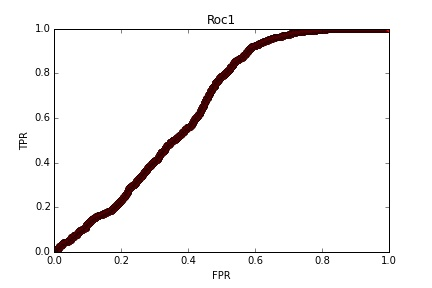
\includegraphics[scale=0.58]{roc1.jpg}
	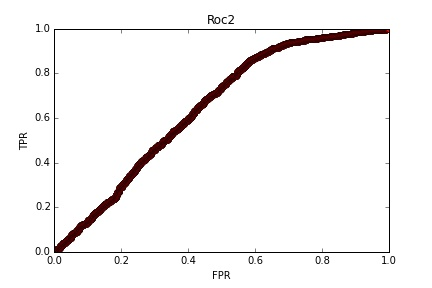
\includegraphics[scale=0.58]{roc2.jpg}\\
	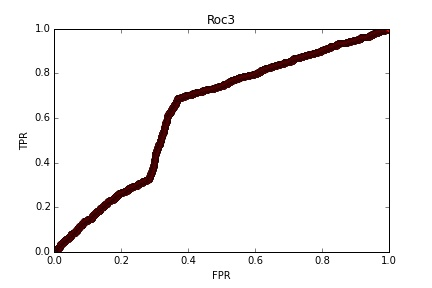
\includegraphics[scale=0.58]{roc3.jpg}		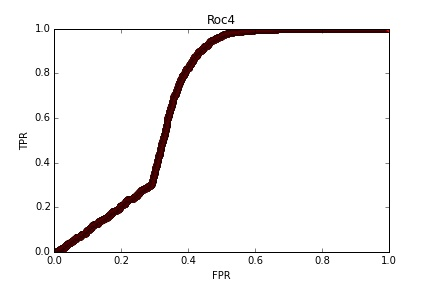
\includegraphics[scale=0.58]{roc4.jpg}
	\caption{ROC for all the predictions.}
\end{figure}
We can notice from the previous figures that Roc4 give a good prediction for TP and minimum FP compared to others.

\begin{lstlisting}[language=R]
AUCROC1 = sum([x[0] for x in roc1cm])
AUCROC2 = sum([x[0] for x in roc2cm])
AUCROC3 = sum([x[0] for x in roc3cm])
AUCROC4 = sum([x[0] for x in roc4cm])
print AUCROC1/3000,AUCROC2/3000,AUCROC3/3000,AUCROC4/3000
\end{lstlisting}
The previous code give the following result :
\[AUC1=0.589976131687,AUC2= 0.587792866941,AUC3= 0.577493004115,AUC4= 0.617289437586\]
\section*{Third Question}

\section*{Fourth Question}
\section*{Fifth Question}
\section*{Sixth Question}
\begin{thebibliography}{9}
	\bibitem{1}
	\href{https://en.wikipedia.org/wiki/Receiver_operating_characteristic}{receiver operating Characteristics }
\end{thebibliography}
\end{document}
